%%%%%%%%%%%%%%%%%%%%%%%%%%%%%%%%%%%%%%%%%
% Stylish Article
% LaTeX Template
% Version 2.1 (1/10/15)
%
% This template has been downloaded from:
% http://www.LaTeXTemplates.com
%
% Original author:
% Mathias Legrand (legrand.mathias@gmail.com) 
% With extensive modifications by:
% Vel (vel@latextemplates.com)
%
% License:
% CC BY-NC-SA 3.0 (http://creativecommons.org/licenses/by-nc-sa/3.0/)
%
%%%%%%%%%%%%%%%%%%%%%%%%%%%%%%%%%%%%%%%%%

%----------------------------------------------------------------------------------------
%	PACKAGES AND OTHER DOCUMENT CONFIGURATIONS
%----------------------------------------------------------------------------------------

\documentclass[fleqn,10pt]{SelfArx} % Document font size and equations flushed left

\usepackage[english]{babel} % Specify a different language here - english by default

\usepackage{lipsum} % Required to insert dummy text. To be removed otherwise

\usepackage{tikz}

%----------------------------------------------------------------------------------------
%	COLUMNS
%----------------------------------------------------------------------------------------

\setlength{\columnsep}{0.55cm} % Distance between the two columns of text
\setlength{\fboxrule}{0.75pt} % Width of the border around the abstract

%----------------------------------------------------------------------------------------
%	COLORS
%----------------------------------------------------------------------------------------

\definecolor{color1}{RGB}{0,0,90} % Color of the article title and sections
\definecolor{color2}{RGB}{0,20,20} % Color of the boxes behind the abstract and headings

%----------------------------------------------------------------------------------------
%	HYPERLINKS
%----------------------------------------------------------------------------------------

\usepackage{hyperref} % Required for hyperlinks
\hypersetup{hidelinks,colorlinks,breaklinks=true,urlcolor=color2,citecolor=color1,linkcolor=color1,bookmarksopen=false,pdftitle={Title},pdfauthor={Author}}

%----------------------------------------------------------------------------------------
%	ARTICLE INFORMATION
%----------------------------------------------------------------------------------------

\JournalInfo{F20RO Intelligent Robotics} % Journal information
\Archive{Robotics Project} % Additional notes (e.g. copyright, DOI, review/research article)

\PaperTitle{Elevated Plus Maze} % Article title

\Authors{Clarissa Cremona\textsuperscript{1}, Helmi Fraser\textsuperscript{2}} % Authors


\affiliation{} % Corresponding author

\Keywords{} % Keywords - if you don't want any simply remove all the text between the curly brackets
\newcommand{\keywordname}{Keywords} % Defines the keywords heading name

%----------------------------------------------------------------------------------------
%	ABSTRACT
%----------------------------------------------------------------------------------------
\addto\captionsenglish{%
	\renewcommand{\abstractname}{}
}
 \Abstract{\textbf{Group 5}: \textsuperscript{1} cc531@hw.ac.uk, \textsuperscript{2} hmf30@hw.ac.uk}

%----------------------------------------------------------------------------------------

\begin{document}

\flushbottom % Makes all text pages the same height

\maketitle % Print the title and abstract box



%----------------------------------------------------------------------------------------
%	ARTICLE CONTENTS
%----------------------------------------------------------------------------------------

\section{Introduction} % The \section*{} command stops section numbering
\addcontentsline{toc}{section}{Introduction} % Adds this section to the table of contents
test




\section{Methods}
\begin{figure*}[ht]\centering
	\def\layersep{2cm}
	\def\hiddenlayers{1}
	\def\hiddenneurons{2}
	
	\def\hiddenlayernodes{3}
	
	\begin{tikzpicture}[shorten >=1pt,->,draw=black!50, node distance=\layersep]
	\tikzstyle{every pin edge}=[<-,shorten <=1pt]
	\tikzstyle{neuron}=[circle,fill=black!25,minimum size=17pt,inner sep=0pt]
	\tikzstyle{input neuron}=[neuron, fill=cyan!50];
	\tikzstyle{output neuron}=[neuron, fill=black!50];
	\tikzstyle{hidden neuron}=[neuron, fill=purple!50];
	\tikzstyle{annot} = [text width=4em, text centered]
	
	% Draw the input layer nodes
	\foreach \name / \y in {0,...,7}
	% This is the same as writing \foreach \name / \y in {1/1,2/2,3/3,4/4}
	\node[input neuron, pin=left:IR Sensor \#\y] (I-\name) at (0,-\y) {};
	
	% Draw the hidden layer nodes
	\foreach \name / \y in {0,...,\hiddenlayernodes}
	\path[yshift=-2cm]
	node[hidden neuron] (H-\name) at (\layersep,-\y cm) {};
	
	
	% Draw the output layer node
	\node[yshift=0][output neuron,pin={[pin edge={->}]right:Left Speed}, right of=H-1] (O-1) {};
	\node[yshift=0][output neuron,pin={[pin edge={->}]right:Right speed}, right of=H-2] (O-2) {};
	
	% Connect every node in the input layer with every node in the
	% hidden layer.
	\foreach \source in {0,...,7}
	\foreach \dest in {0,...,\hiddenlayernodes}
	\path (I-\source) edge (H-\dest);
	
	
	% Connect every node in the second hidden layer with the output
	\foreach \source in {0,...,\hiddenlayernodes}
	\foreach \dest in {1,...,2}
	\path (H-\source) edge (O-\dest);
	
	% Annotate the layers
	\node[xshift=0cm][annot,above of=I-1] (first) {Input layer};
	\node[xshift=1cm][annot,right of=first, node distance=1cm] (hl) {Hidden layer};
	\node[xshift=1cm][annot,right of=hl, node distance=1cm] (ll) {Output layer};
	\end{tikzpicture}
	\caption{Neural network}
	\label{fig:NN}
\end{figure*}
%------------------------------------------------

\begin{figure*}[ht]\centering % Using \begin{figure*} makes the figure take up the entire width of the page
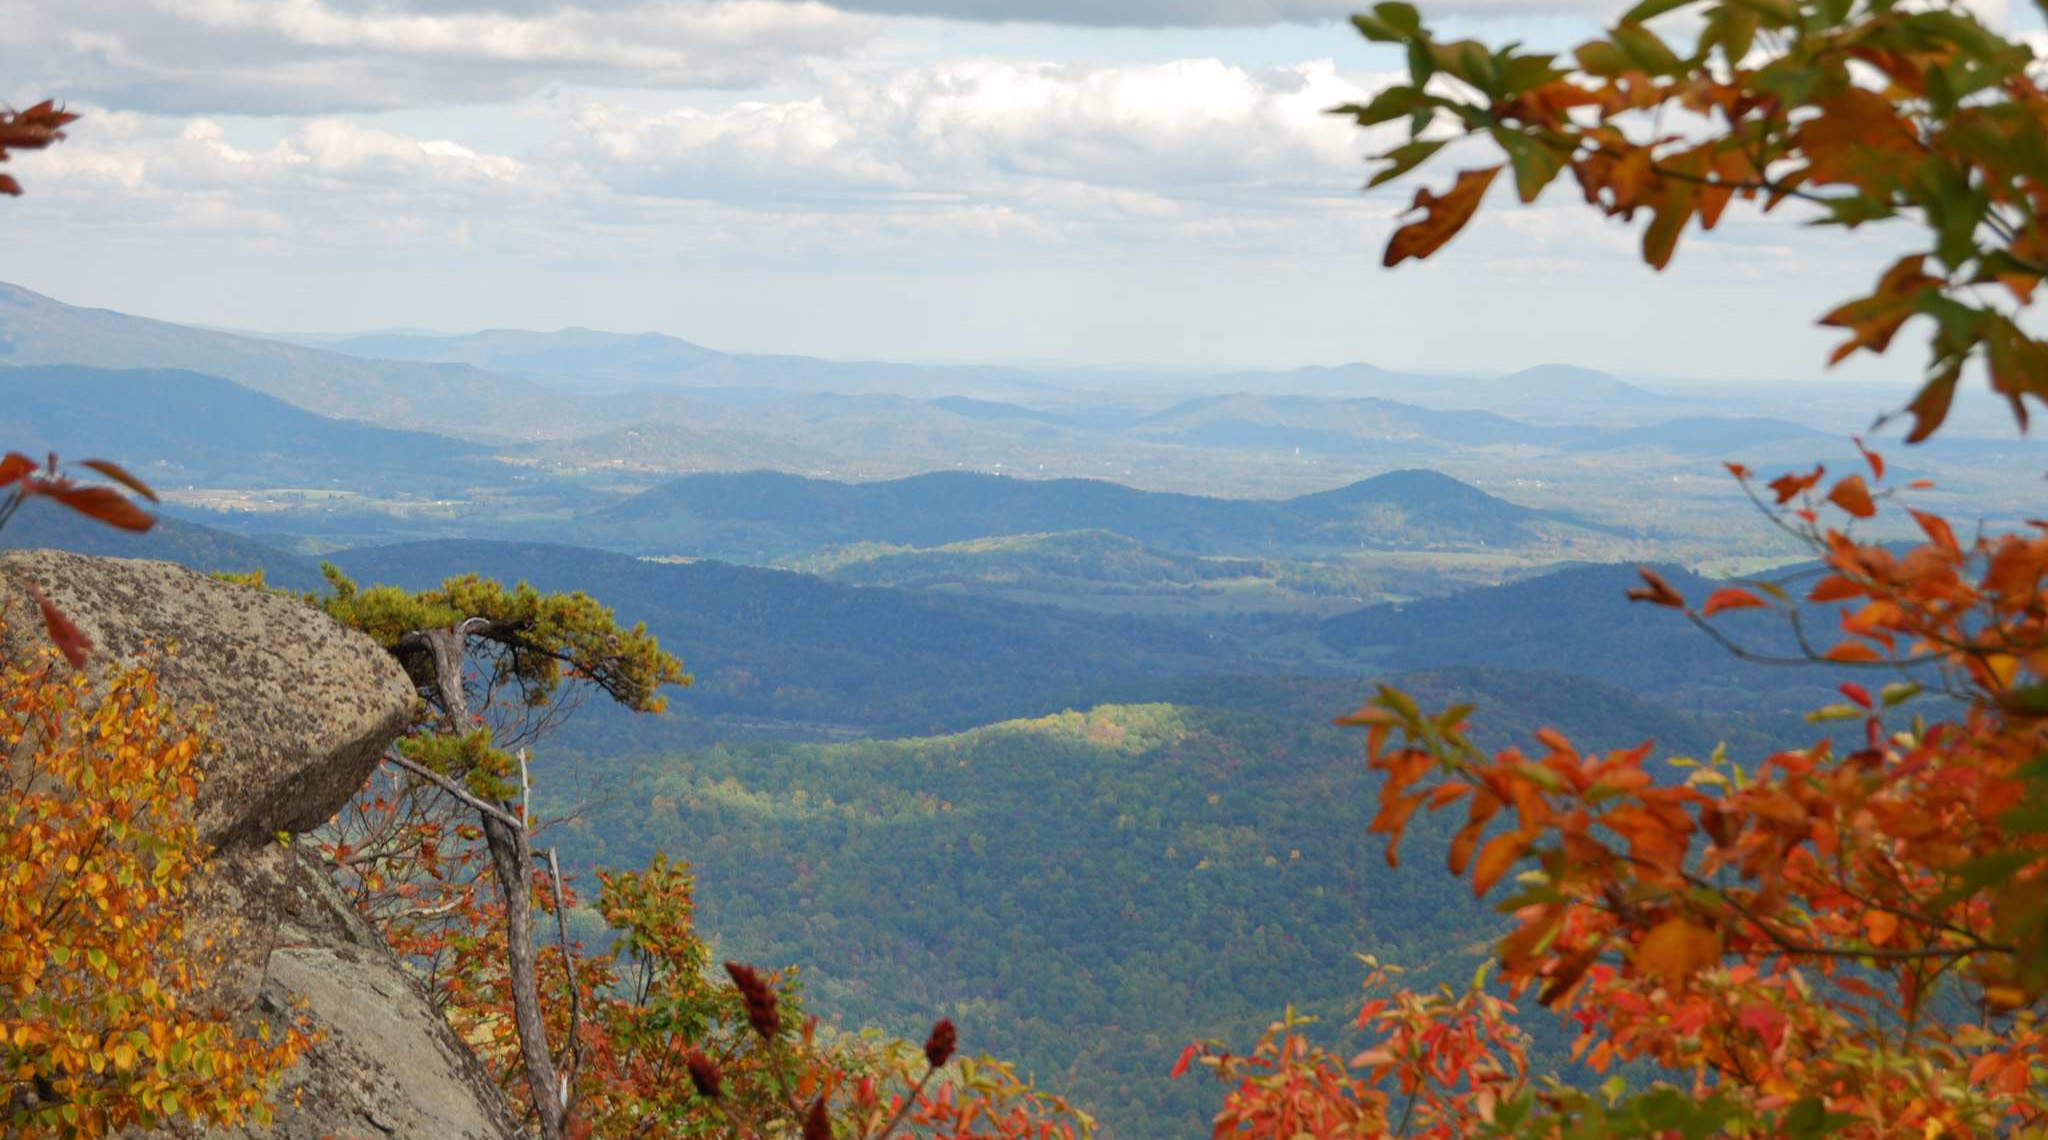
\includegraphics[width=\linewidth]{view}
\caption{Wide Picture}
\label{fig:view}
\end{figure*}



\begin{equation}
\cos^3 \theta =\frac{1}{4}\cos\theta+\frac{3}{4}\cos 3\theta
\label{eq:refname2}
\end{equation}



\begin{enumerate}[noitemsep] % [noitemsep] removes whitespace between the items for a compact look
\item First item in a list
\item Second item in a list
\item Third item in a list
\end{enumerate}

\subsection{Subsection}

\lipsum[6] % Dummy text

\paragraph{Paragraph} \lipsum[7] % Dummy text
\paragraph{Paragraph} \lipsum[8] % Dummy text

\subsection{Subsection}

\lipsum[9] % Dummy text

\begin{figure}[ht]\centering
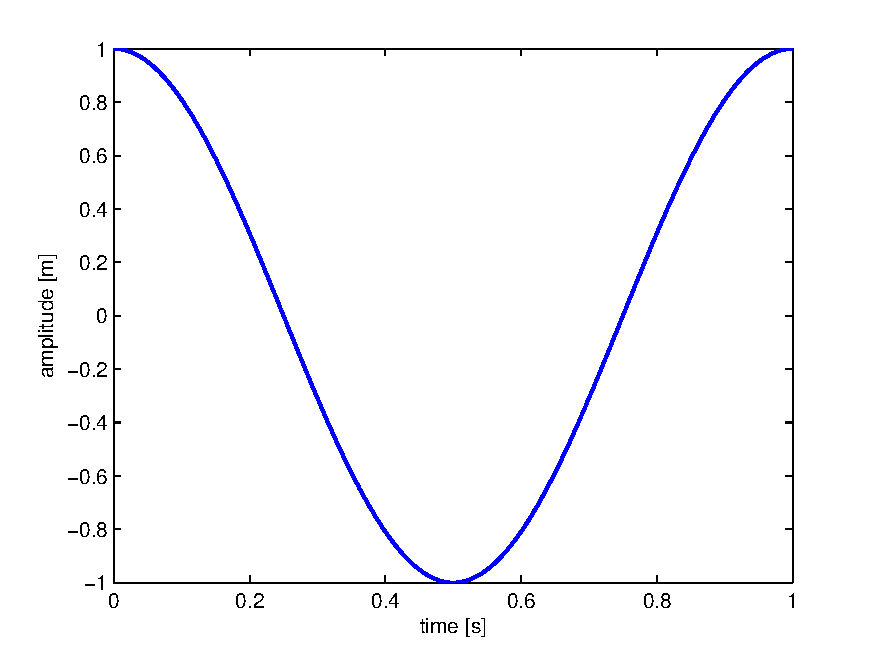
\includegraphics[width=\linewidth]{results}
\caption{In-text Picture}
\label{fig:results}
\end{figure}

Reference to Figure \ref{fig:results}.

%------------------------------------------------

\section{Results and Discussion}

\lipsum[10] % Dummy text

\subsection{Subsection}

\lipsum[11] % Dummy text

\begin{table}[hbt]
\caption{Table of Grades}
\centering
\begin{tabular}{llr}
\toprule
\multicolumn{2}{c}{Name} \\
\cmidrule(r){1-2}
First name & Last Name & Grade \\
\midrule
John & Doe & $7.5$ \\
Richard & Miles & $2$ \\
\bottomrule
\end{tabular}
\label{tab:label}
\end{table}

\subsubsection{Subsubsection}

\lipsum[12] % Dummy text

\begin{description}
\item[Word] Definition
\item[Concept] Explanation
\item[Idea] Text
\end{description}

\subsubsection{Subsubsection}

\lipsum[13] % Dummy text

\begin{itemize}[noitemsep] % [noitemsep] removes whitespace between the items for a compact look
\item First item in a list
\item Second item in a list
\item Third item in a list
\end{itemize}

\subsubsection{Subsubsection}

\lipsum[14] % Dummy text

\subsection{Subsection}

\lipsum[15-23] % Dummy text

%------------------------------------------------
\phantomsection
\section*{Acknowledgments} % The \section*{} command stops section numbering

\addcontentsline{toc}{section}{Acknowledgments} % Adds this section to the table of contents

So long and thanks for all the fish \cite{Figueredo:2009dg}.

%----------------------------------------------------------------------------------------
%	REFERENCE LIST
%----------------------------------------------------------------------------------------
\phantomsection
\bibliographystyle{unsrt}
\bibliography{sample}

%----------------------------------------------------------------------------------------

\end{document}